\section{Measurement and Evaluation}
\label{sec:eval}
\textbf{Data.} A GitHub Actions run on \measureDate\ listed the labeler directory, probed every endpoint once, and replayed each labeler's full label stream with \texttt{subscribeLabels} from sequence zero. For the \windowedN services whose stream had passed sequence number three million, only the last three million sequence numbers were replayed. An earlier run from a second vantage point (our cloud workspace) gave nearly the same reachability (\altAnswering answering, \altBrowser browser-readable), so the failures below are the services', not the vantage point's. The author set the topic and the direction of the experiments; an AI assistant (Anthropic Claude) helped carry them out and analyse them.

\textbf{Reachability.} Of \labDeclared accounts that declare a labeler, \labEndpoint publish an endpoint, but only \labAnswering (\labAnsweringPct\%) answer a \texttt{queryLabels} request; the rest cannot be reached (\labConnFail), fail TLS (\labTlsFail) or answer with an HTTP error or a body that is not JSON (\labHttpFail). Of the answering services, \labBrowser (\labBrowserPctOfAnswering\%) send a CORS header. A browser-only client such as a third-party app or LabelLens itself therefore sees at most \labBrowserPctOfEndpoint\% of declared endpoints, which is why the census needs its snapshot fallback.

\begin{figure}[t]
  \centering
  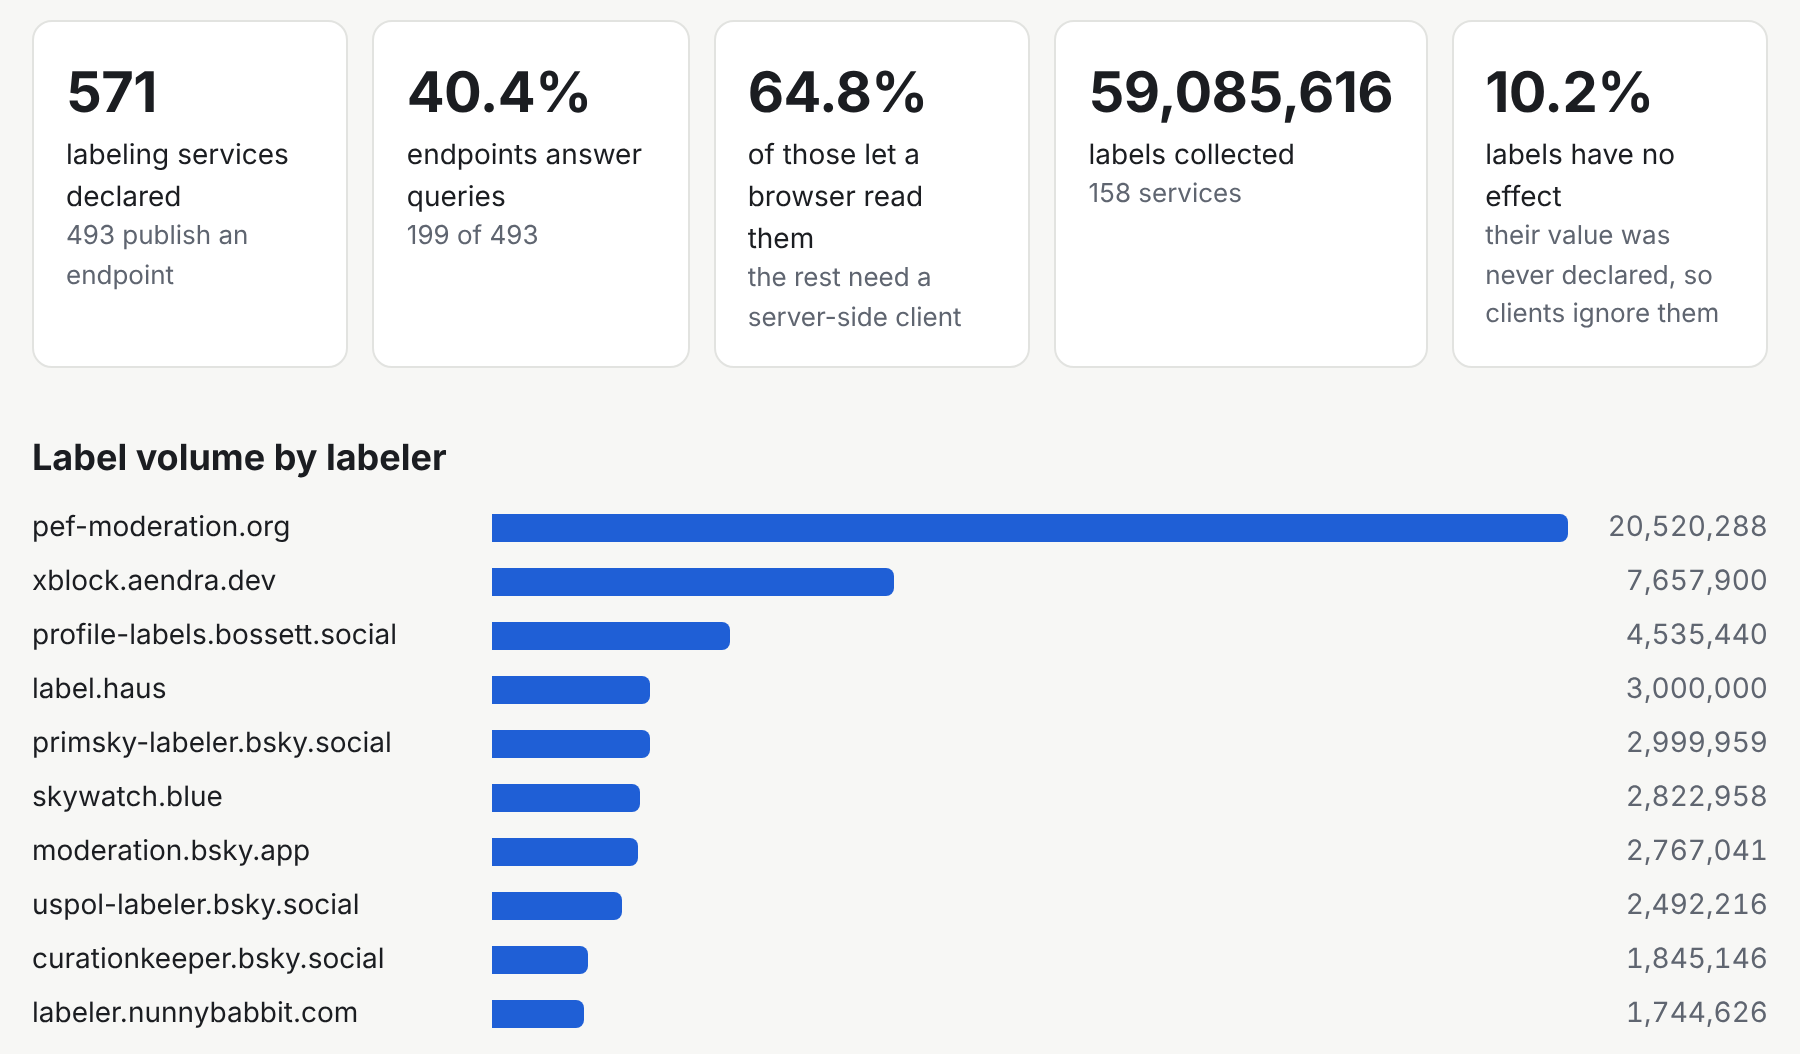
\includegraphics[width=\columnwidth]{figures/ui_network.png}
  \caption{The Network page (\measureDate): summary tiles and the ten services with the most labels. Services whose stream had passed sequence number three million, such as \texttt{moderation.bsky.app}, were replayed from a recent window, so their bars count that window only.}
  \label{fig:network}
  \Description{Five summary tiles (571 labeling services declared, 40.4\% of endpoints answer, 64.8\% of those browser-readable, 59 million labels collected, 10.2\% of labels have no effect) above a horizontal bar chart of label volume for the ten largest labelers.}
\end{figure}

\textbf{Labels.} We collected \labLabelsM million labels from \labCollected services (\labPostPct\% on posts, \labAccountPct\% on accounts). Volume is concentrated: the five largest services issued \labTopFivePct\% of all labels. \labInertPct\% of labels carry a value their labeler never declared; clients drop such labels silently, and for \labInertMajority services they are the majority. \labRetractedPct\% of (subject, value) pairs end retracted. Protective labelers differ widely in speed: among the \latN with at least 100 post labels, the median time from post creation to label is under ten seconds for \latFastN (automated classifiers) and over an hour for \latSlowN.

\textbf{Overlap and divergence.} Stacks rarely agree because they rarely overlap: of the \accProtM million accounts labelled by any protective labeler, \accTwoPlusPct\% are labelled by two or more. To measure what this means for readers, we drew a uniform sample of labelled subjects (a subject is kept when its hash is 0 modulo 1{,}000; \lensPostN posts and \lensAcctN accounts) and evaluated each lens offline with the same moderation code as the site (Table~\ref{tab:lens}). For posts, the protective stack changes the presentation of \lensPostProtDiffPct\% relative to a logged-out visitor, mostly by adding an info badge, while the popular stack changes only \lensPostPopDiffPct\%: the most-liked labelers are mostly descriptive (badges, interests, verification), so popularity is a poor guide to protection. The effect is also concentrated: \lensTopDriverPct\% of the changed posts are changed by one service, \texttt{\lensTopDriver}, which flags links to other platforms and suspected disinformation sources. Which labelers a user adds matters more than how many, and this is exactly what the census and the editable stack expose for a single item. Subscribing to the labelers that labelled the item (at most twenty) changes \lensPostAllDiffPct\% of posts.

\begin{table}[t]
  \caption{How labelled items are shown under each lens (uniform sample; percent of items).}
  \label{tab:lens}
  \small
  \begin{tabular}{@{}lrrrr@{}}
    \toprule
    Lens & Hidden & Warned & Info badge & As is \\
    \midrule
    \lensTableRows
    \bottomrule
  \end{tabular}
\end{table}

\textbf{Census performance.} We tried \censusTried items (posts and accounts from the sample) in headless Chromium from our workspace; \censusGone sampled posts had since been deleted or hidden, and the other \censusN were inspected. The lenses appeared after \censusMedian\,s at the median (\censusMax\,s at most); the recheck of slow services and of those offline at measurement time finished after \censusTotalMedian\,s and added at most \censusRevivedMax answers. At least \censusLive labelers answered live on every run, and \snapSources more through the full snapshot.
